\chapter{Sensors}
To understand how sensors work, this section provides an overview of the colour coding of the sensors and the circuit diagram of each sensor used in the project.

\begin{figure}
    \centering
    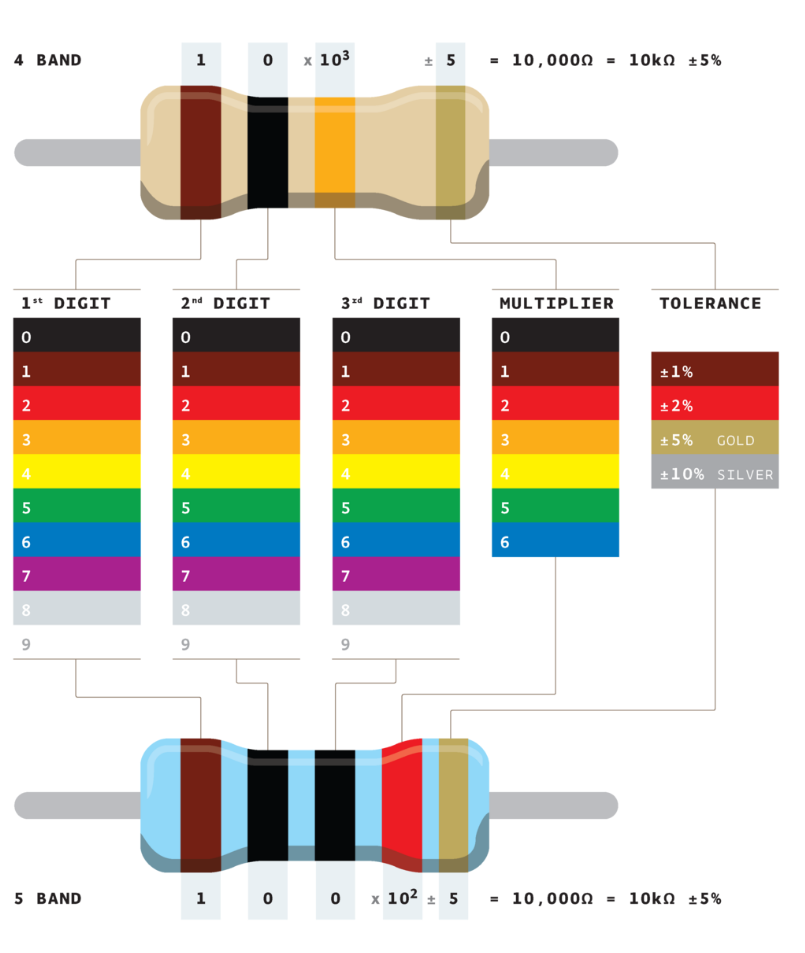
\includegraphics[width=0.5\linewidth]{images/sensors-color-code.png}
    \caption{ Colour codes in sensors \cite{36}}
    \label{fig:sensors-color-code}
\end{figure}

\section{Pulse Sensor Circuit}
Figure \ref{fig:pulse-sensor} shows the internal circuit diagram of a pulse sensor. It consists of an optical heartbeat sensor, an amplification circuit, and a noise cancellation circuit.

\begin{figure}
    \centering
    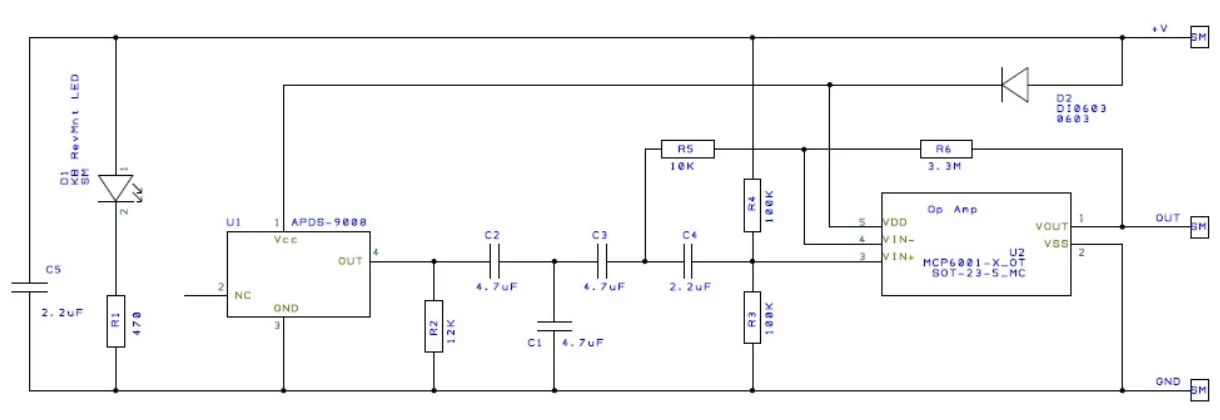
\includegraphics[width=0.75\linewidth]{images/image.png}
    \caption{Internal block diagram of an SEN-11574 pulse sensor \cite{37}}
    \label{fig:pulse-sensor}
\end{figure}

\section{LM-35 Sensor Circuit}
Figure \ref{fig:lm-35-sensor} shows the internal circuit diagram of a LM-35 sensor. In the figure, A1 shows the input where it senses the temperature and A2 provides the output voltage of the circuit. The circuit is made in such a way that it outputs a voltage proportional to the temperature it measures. This makes it easier to calculate the temperature of body eliminating electronic complexities. 

\begin{figure}
    \centering
    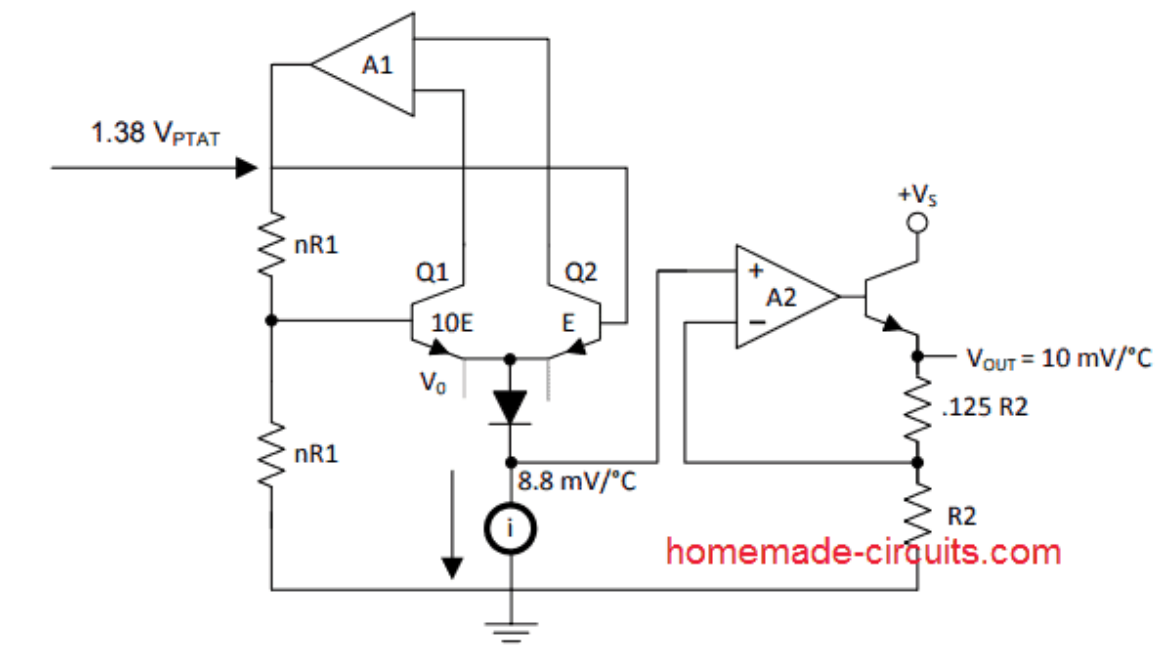
\includegraphics[width=0.5\linewidth]{images/lm-35.png}
    \caption{Internal block diagram of IC LM-35 Sensor \cite{38}}
    \label{fig:lm-35-sensor}
\end{figure}
